\documentclass{article}

\usepackage{amsmath, amssymb}
\usepackage{mathtools}
\usepackage{graphicx}

\newcommand{\dx}{\, dx}
\newcommand{\dy}{\, dy}
\newcommand{\dA}{\, dA}
\newcommand{\du}{\, du}
\newcommand{\dw}{\, dw}

\title{Interesting Examples in Undergraduate Mathematics}
\author{Matthew McGonagle}

\begin{document}

\maketitle

\tableofcontents

\section{Introduction}

The purpose of these notes is examples in undergraduate mathematics that the author considers to be interesting; this could be from applications or pure mathematical interest. 

\section{One Variable Differential Calculus}

\subsection{Gauss and the Gauss Distribution}

\subsubsection*{History}

A good reference on the history of the gaussian distribution is \cite{gaussian}.

The history of how to deal with errors is intimately tied to astronomy; astronomical predictions involve quantities that need to be measured to high precision. 
Practical limits force astronomers to deal with the errors of predictions or measurements never being in complete agreement.

In the 18th century and early 19th century, there was some confusion as to how to deal with these errors in measurement. 
As an example, there was some dispute as to whether to use the average or the median of measurements. 
One of the problems was a theoretical foundation for understanding error was in its infancy. 
For example, Laplace created a model of typical error that is far from the typical gaussian distribution considered today.

So how did Gauss arrive at his distribution? First it should be noted that he worked on modeling error while solving a problem in astronomy. 
On January 1, 1801, Giuseppe Piazzi observed the Ceres asteriod. 
He was interested in whether Ceres was a new planet, but he could only take a small number of observations of its position before it disappered behind the sun. 
Ceres was estimated to be visible again after about a year, which left many astronomers with the question of where to find it in the sky.

Gauss greatly increased his reputation by correctly solving this problem; in fact, his correct answer was actually in disagreement with most reputable astronomers. 
Aside from his masterful use of geometry, part of his solution is how to deal with the errors in measurements that were made. 
It is this problem that lead him to the gaussian distribution as a model for the error.

His approach to modeling the error is the following.

He considers the errors to be random described by a differentiable probability density \(p(x)\). The distribution of the errors should satisfy the following:

\begin{enumerate}
\item Smaller errors are more probable, i.e. the density \(p(x)\) should have a maximum at \(x = 0\).
\item The distribution of errors should symmetric, i.e. \(p(-x) = p(x)\).
\item Consider any observed quanitity \(X\) with true value \(X_0\) and errors modeled by our distribution, i.e. \(X = X_0 + G\) where \(P(G = x) = p(x)\). 

Given any set of observations \(\{x_1, x_2, ..., x_n\}\), then the likelihood \(P(x_1, x_2, ..., x_n | X_0)\) 
(i.e. the probability of observing \(x_1\), \(x_2\), ... \(x_n\) given the true value is \(X_0\)) is maximized by \(X_0\) being the average of \(\{x_1, x_2, ..., x_n\}\)
(i.e. \(X_0 = \frac{x_1 + x_2 +... + x_n}{n}\)). Let us explain this in a little more detail.

We are assuming that the errors \(\{x_1, x_2, ..., x_n\}\) are independent. So
\begin{equation}
P(x_1, x_2, ..., x_n | X_0) = p(x_1 - X_0)p(x_2 - X_0)...p(x_n - X_0).
\end{equation}
When we speak of maximizing the likelihood, we think of all of the observations \(x_i\) being fixed. So the above is considered to a function of only the one variable \(X_0\). That is,
we are considering the likelihood functions
\begin{equation}
L(X_0) = p(x_1 - X_0)p(x_2 - X_0)...p(x_n - X_0).
\end{equation}
Then our assumption is that the maximum of \(L(X_0)\) occurs at the average of our observations \(X_0 = \frac{x_1 + x_2 + ... + x_n}{n}\).

This amounts to Gauss's justification of using averages over median. He is purposefully choosing a model of error where the average of the observations is the most likely explanation of
the true value.

\end{enumerate}

\subsubsection*{The Problem}

Show that Gauss' requirements on \(p(x)\) force \(p(x)\) to be a Gaussian distribution.

\subsubsection*{The Solution}

First, let us consider condition (3) and the consequences of maximizing the likelihood. First note that \(L(X_0) \geq 0\), so maximizing \(L(X_0)\) is equivalent to maximizing \(f(X_0) = \log(L(X_0))\). 
Using the logarithm will be more convenient as it will turn the product of the \(p(x_i - X_0)\) into a sum of logarithms; so we have  
\begin{equation}
h(X_0) = \log(p(x_1 - X_0)) + \log(p(x_2 - X_0)) + ... + \log(p(x_n - X_0)).
\end{equation}

To find the maximum, let's set the derivative to be zero:
\begin{equation}
0 = h'(X_0) = -\left(\frac{p'(x_1 - X_0)}{p(x_1 - X_0)} + \frac{p'(x_2 - X_0)}{p(x_2 - X_0)} + ... + \frac{p'(x_n - X_0)}{p(x_n - X_0)} \right). 
\end{equation}

Now the key is that condition (3) applies to any possible set of observations, no matter how unprobable. Since \(p(x)\) is continuous with maximum at \(x = 0\), we know that
there exists an interval \([-\delta, \delta]\) around \(x = 0\) such that \(p(x) > 0\) for all \(x \in [-\delta, \delta]\). 
In particular, we know that observations in \([X_0 - \delta, X_0 + \delta]\) are all possible. 
So now consider any real number \(r \in [-\delta, \delta]\) and the observations \(\{x_1 = X_0\}\) and \(\{x_2 = ... = x_n = X_0 + r\}\).

Since we have already fixed \(X_0\) to represent our true value, let us now use \(y\) as the independent variable for our likelihood. So we seek to maximize
\begin{equation}
L(y) = p(x_1 - y) p(x_2 - y) ... p(x_n - y).
\end{equation}
Condition (3) says this maximum is at \(y = \frac{x_1 + x_2 + ... x_n}{n} = X_0 + \frac{n-1}{n} r\). To simplify notation, let \(f(x) = \frac{p'(x)}{p(x)}\). So we get 
\begin{equation} \label{gauss:homog}
0 = f\left(-\frac{n-1}{n} r\right) + (n - 1) f\left(\frac{1}{n} r\right). 
\end{equation}
Now, note that \(p(x)\) symmetric implies that \(p'(x)\) is anti-symmetric. Therefore \(f(x)\) is anti-symmetric. So we get that
\begin{equation}
f\left(\frac{n-1}{n} r\right) = (n-1) f\left(\frac{1}{n} r \right).
\end{equation}

What are the consequences of this equation? Fix any \(r_0\) small enough such that \(2r_0\) is in the interval \([-\delta, \delta]\). Now note that \(\frac{n}{n-1}r_0\) is also in the interval for
any \(n > 1\), and consider \(r = \frac{n}{n-1} r_0\). Then we have that 
\begin{equation}
\frac{1}{n-1} f(r_0) = f\left(\frac{r_0}{n-1}\right).
\end{equation}

Now consider \(0 < k \leq n + 1\). Note that \(\frac{k}{n}r \) is in the interval too, and now apply \ref{gauss:homog} for \(n -> k\) and \(r -> \frac{k}{n} r\), we get
\begin{equation}
f\left(\frac{k-1}{n}r\right) = (k-1)f\left(\frac{1}{n}r\right).
\end{equation} 
So for any fraction of the form \(frac{m}{n}\) where \(0 < m \leq n\), we have that
\begin{equation}
f\left(\frac{m}{n} r_0\right) = \frac{m}{n} f(r_0). 
\end{equation}

Consider the function \(g(x) = f(r_0) x\). We have that \(g(x) - f(x) = 0\) for any \(x\) that is a rational multiple of \(r_0\) and \(0 < |x| \leq r_0\). Hence, by the continuity of \(f(x)\), 
we have that \(f(x) = g(x) = f(r_0) x\) for all \(|x| \leq r_0\).

Therefore, we may write that \(f(x) = k x\) for some constant \(k\) and \(x\) on some interval around zero. This gives us the differential equation 
\begin{equation}
\frac{p'(x)}{p(x)} = k, 
\end{equation}
locally around \(x = 0\). Integrating we get
\begin{equation}
\log(p(x)) = \frac{k}{2}x^2 + C. 
\end{equation} 
This can be written in the form \(p(x) = Ae^{-Bx^2}\). So we see the probability distribution extends to be non-zero on all \(x\). 
Furthermore, the constants \(A\) and \(B\) can be related 
by the fact that \(p(x)\) is a probability density so that \(\int_{-\infty}^{\infty} Ae^{-Bx^2} \dx = 1\). It is standard to solve for \(A\) in terms of \(B\).

To solve \(\int_{-\infty}^{\infty} e^{-Bx^2} \dx\), we square the integral and switch to polar coordinates to get
\begin{equation}
\int\limits_{-\infty}^\infty e^{-Bx^2} \dx = \sqrt{\frac{\pi}{B}}.
\end{equation}
So we get that \(A = \sqrt{\frac{B}{\pi}}\), and then
\begin{equation}
p(x) = \sqrt{\frac{B}{\pi}} e^{-Bx^2}. 
\end{equation}

\subsection{The Schwarzian Derivative}

In this example we will derive the form of the Schwarzian derivative \(Su\) for a smooth function \(u:\mathbb R \to \mathbb R\)
given by
\begin{equation}
Su = \frac{u'''}{u'} - \frac{3}{2}\left(\frac{u''}{u'}\right)^2.
\end{equation}
What is special about the Schwarzian derivative is that you get the same result if you apply it to
a function \(w\) that is a linear fractional transformation of \(f\), i.e. for
\begin{equation}
w(x) = \frac{A + Bu(x)}{C + Du(x)},
\end{equation}
for constants \(A, B, C,\) and \(D\), we have that \(Su = Sw\). We will first briefly discuss 
linear fractional transformations and then how we aim to derive the Schwarzian derivative from the
above invariance property.

A nice introductory reference to the Schwarzian derivative and its relationship to projective differential geometry
is \cite{schwarzian}.

\subsubsection*{The Setup: Linear Fractional Transformations}

A linear fractional transformation for one real variable is a function of the form
\begin{equation}
T(y) = \frac{A + By}{C + Dy},
\end{equation}
for constants \(A, B, C\) and \(D\). Note that the function is not defined for the single point \(C + Dy = 0\) when
\(D\neq 0\).

An important motivation for linear fractional transformations is perspective transformations. First imagine an
eye sitting at the origin in \(\mathbb R^2\), and the eye is looking down the x-axis towards \(+\infty\). 
Everything the eye
observes is equivalent to seeing something sitting in its viewing line (or plane for 3-dimensions). We will
take the viewing line of the eye to be \(\{x = 1\}\). See the figure below.

\begin{figure}[h]
\centering
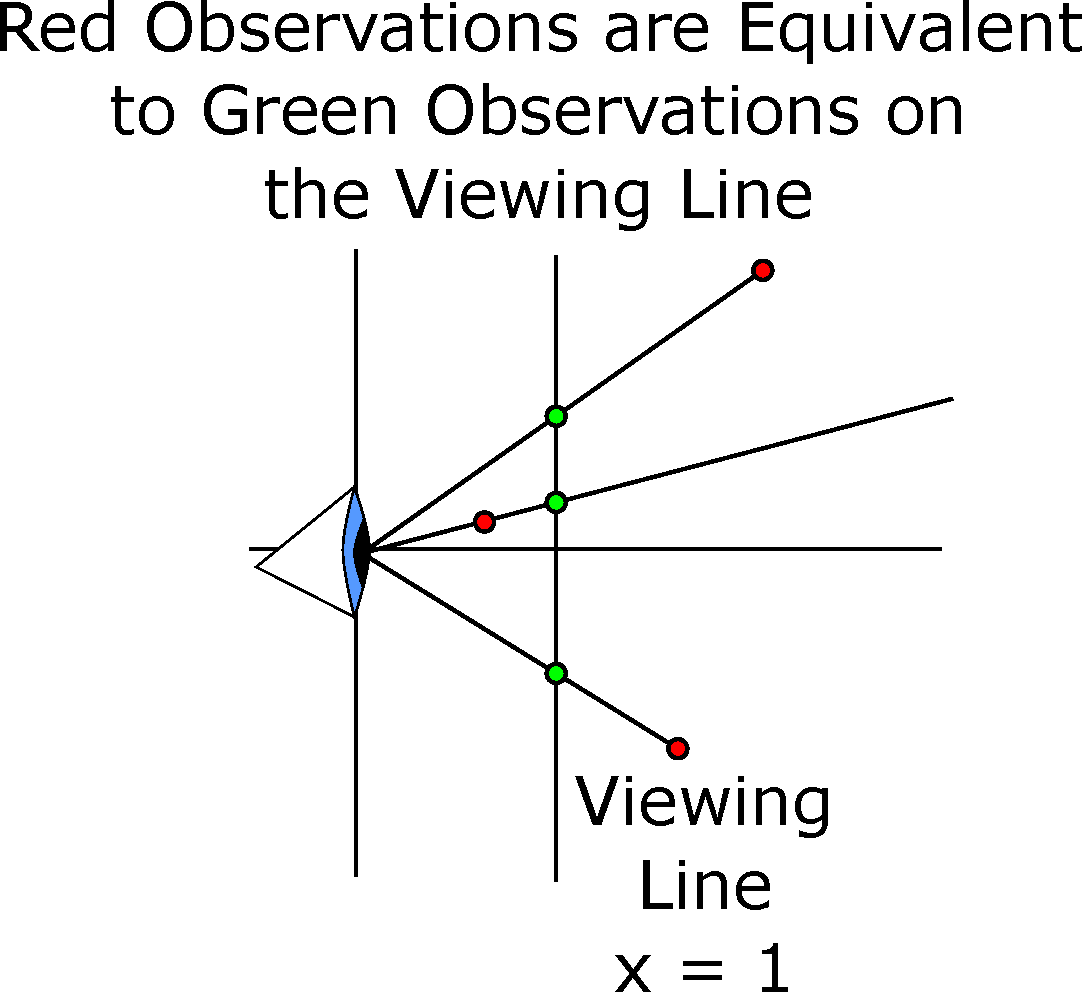
\includegraphics[width = 2in]{oneVarDiffCalc/perspective1.pdf}
\end{figure}

Now imagine that the eye rotates \(\pi/4\) radians counter-clockwise; it is now looking down a line that makes
an angle of \(\pi/4\) radians with the x-axis. Furthermore, its viewing line has rotated to be the 
line \(\left\{y + x = 2\sqrt{\frac{1}{2}} \right\}\). Let \(\tilde y\) denote the position along this 
new viewing line. See the figure below

\begin{figure}[h]
\centering
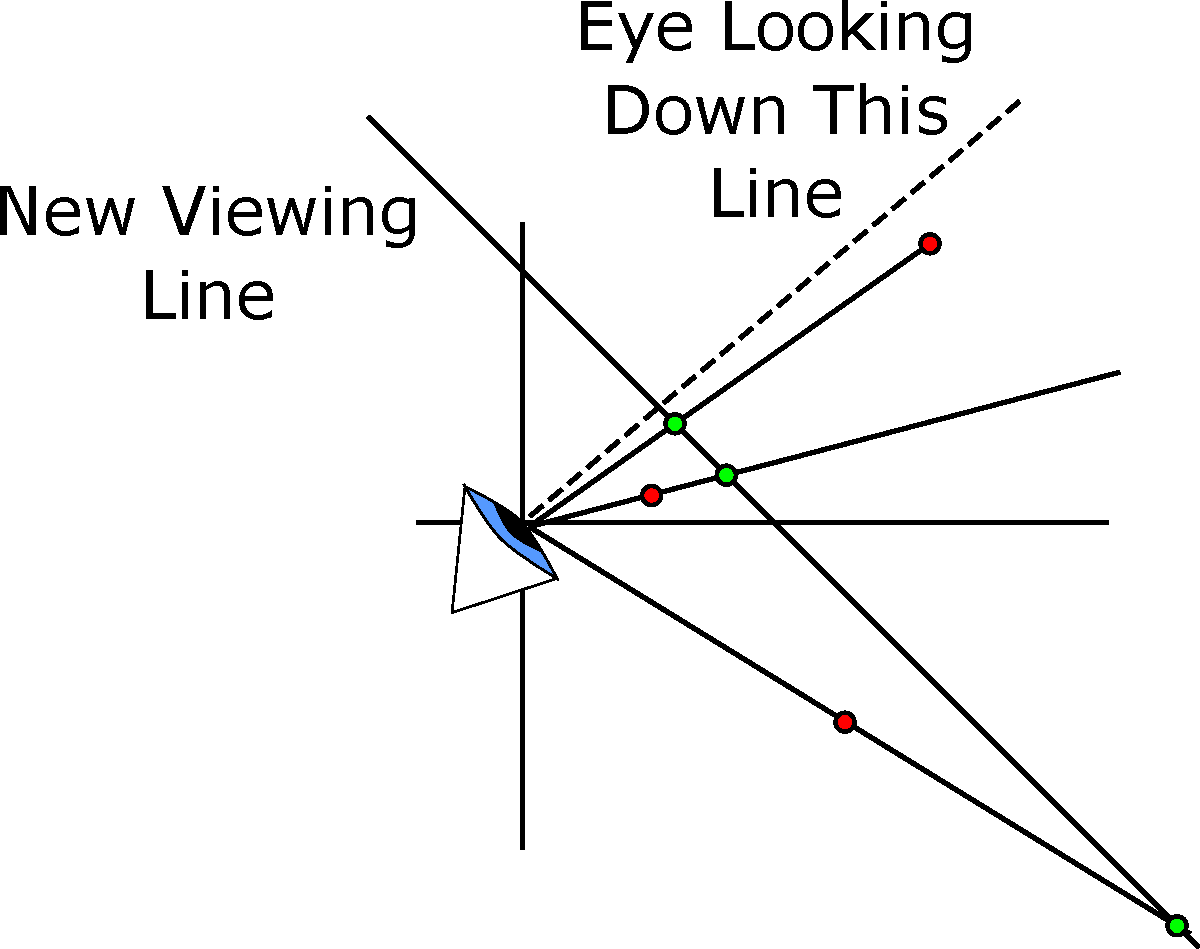
\includegraphics[width = 2in]{oneVarDiffCalc/perspective2.pdf}
\end{figure}

Let \(\tilde y\) measure position on the viewing line relative the line \(\{y = x\}\), i.e. the line that eye is
looking down. If an object appears to be at a point \(y\) on the original viewing line, what is its new position \(\tilde y\) on 
the new viewing line?
The answer turns out to be a linear fractional transformation, i.e.
\begin{equation}
\tilde y = \frac{A + By}{C + Dy},
\end{equation} 
for some constants \(A, B, C,\) and \(D\) depending on the angle of rotation.

Linear fractional transformations are also a classical topic in complex analysis, projective geometry, and
conformal geometry.

\subsubsection*{Finding the Schwarzian Derivative}

Now we will discuss our method of finding the Schwarzian derivative \(Su\) of a function \(u: \mathbb R \to 
\mathbb R\). We will demand that \(Su\) has the following properties:

\begin{enumerate}
\item The Schwarzian derivative is defined by
\begin{equation}
Su = F(u, u', u'', u'''),
\end{equation}
for some function \(F(a, b, c, d)\).

\item Given any function \(u(x)\) and linear fractional transformation \(T(y) = \frac{A + By}{C + Dy}\), we have
that the function defined by
\begin{equation}
w(x) = T(u(x)) = \frac{A + Bu(x)} {C + Du(x)},
\end{equation}
satisfies \(Sw = Su\).
\end{enumerate}

You can interpret the Schwarz derivative via perpective transformations. Suppose there is a particle moving in a
2-dimensional plane and the eye from our first set-up in the previous section observes it at position \(u(t)\)
in its viewing line. Next, suppose another observer is at 45 degrees relative to the first observer (so the 
second set-up) and observes the particle at position \(w(t)\) on their viewing line. Furthermore, suppose
neither observer knows the distance of their viewing plane and doesn't know the angle difference of
their perspectives. Is there some measure of the rate of change in the particle's position that they can agree on?

Yes, the Schwarzian derivative. Their observations differ by some linear fractional transformation; 
since they are missing data on their perspectives, they can't reconstruct the actual position of the particle
and they also can not reconstruct the details of the linear fractional transformation that relates their observations.
However, the Schwarzian derivative will always be the same despite no knowing the exact transformation. It is
enough to just know that it is a linear fractional transformation. 

\subsubsection*{The Problem}

Given the two properties of the Schwarzian derivative listed above, show that
\begin{equation}
F(u, u', u'', u''') = J\left( \frac{u'''}{u'} - \frac{3}{2} \left(\frac{u''}{u'}\right)^2 \right),
\end{equation}
for some function \(J\). Thus, deduce that a reasonable definition of the Schwarzian derivative is
\begin{equation}
Su = \frac{u'''}{u'} - \frac{3}{2}\left( \frac{u''}{u'} \right)^2.
\end{equation} 

\subsubsection*{The Solution}

First, we start by looking at the consequences of having an invariant for translations \(T(y) = A + y\) which
are fractional transformations for \(B = 1, C = 1,\) and \(D = 0\). Note that the derivatives of \(u\) and \(w\)
are equal. So we get that for any function \(u\) that
\begin{equation}
F(u + A, u', u'', u''') = F(u, u', u'', u''').
\end{equation}
Now, note that for any point \((a, b, c, d)\), we can find a function \(u\) such that 
\((u, u', u'', u''') = (a,b,c,d)\) for some point \(x\). So we get that
\begin{equation}
F(a + A, b, c, d) = F(a, b, c, d),
\end{equation} 
for any \(A, a, b, c,\) and \(d\). In particular, since we can vary \(A\) without changing the right
hand side, we see that the value \(F(a, b, c, d)\) is actually independent of \(a\). Therefore, we
may find a function \(G(b, c, d)\) such that
\begin{equation}
F(a, b, c, d) = G(b, c, d).
\end{equation}
Note that \(G(u', u'', u''')\) will be invariant for linear fractional transformations of \(u\) and 
that \(G(u', u'', u''')\) depends only on the derivatives of \(u\).

Next, we consider the effect of scalings \(T(y) = By\), these are also a specific class of linear fractional
transformations. We have that
\begin{equation}
G(Bu', Bu'', Bu''') = G(u', u'', u'''),
\end{equation}
for any \(B\). Similar to before, we get that
\begin{equation}
G(Bb, Bc, Bd) = G(b, c, d),
\end{equation}
for any \(B, b, c,\) and \(d\). Therefore, we see that \(G\) must be homogeneous of degree 0, i.e.
\begin{equation}
G(\lambda b, \lambda c, \lambda d) = G(b, c, d),
\end{equation}
for any constant scaling \(\lambda\).

Next, we consider the specific linear fractional transformation \(T(y) = \frac{1}{y}\). We then have that
\begin{align}
w & = \frac{1}{u}, \\
w' & = -\frac{u'}{u^2}, \\
w'' & = \frac{2u'^2}{u^3} - \frac{u''}{u^2}, \\
w''' & = \frac{6u'u''}{u^3} - \frac{6u'^3}{u^4} - \frac{u'''}{u^2}. 
\end{align}
So from the invariance of \(G\), we get that
\begin{equation}
G(u', u'', u''') = G\left( -\frac{u'}{u^2},
    \frac{2u'^2}{u^3} - \frac{u''}{u^2},
    \frac{6u'u''}{u^3} - \frac{6u'^3}{u^4} - \frac{u'''}{u^2} \right). 
\end{equation}
Now use the 0-homoegeneity of \(G\) to get
\begin{equation}
G(u', u'', u''') = G\left(-1, 
    \frac{2u'}{u} - \frac{u''}{u'}, 
    \frac{6u''}{u} - \frac{6u'^2}{u^2} - \frac{u'''}{u'}\right)
\end{equation}
Note that the expression on the right hand side contains terms involving \(u\) without any derivatives,
which isn't directly supplied as an argument to \(G\) on the left hand side. So when like before we
pass to general coordinates, the \(u\) terms turn into general constants \(A\). So we get
\begin{equation}
G(b, c, d) = G\left(-1, 
    \frac{2b}{A} - \frac{c}{b}, 
    \frac{6c}{A} - \frac{6b^2}{A^2} - \frac{d}{b}\right),
\end{equation} 
for any constant \(A\). So there exists a function \(H\) such that
\begin{equation}
G(b, c, d) = H\left(
    \frac{2b}{A} - \frac{c}{b}, 
    \frac{6c}{A} - \frac{6b^2}{A^2} - \frac{d}{b}\right),
\end{equation}
for any constant \(A\).

The fact that \(A\) is any general constant that appears on the right hand side but is not on the left means that 
there is more information to draw from \(H\). Let \(\theta = \frac{2b}{A} - \frac{c}{b}\). So
\begin{align}
\frac{6c}{A} - \frac{6b^2}{A^2} - \frac{d}{b} & = 
    \frac{3c}{b}\left(\theta + \frac{c}{b}\right)
    - \frac{3}{2}\left(\theta + \frac{c}{b}\right)^2 - \frac{d}{b}, \\
& = 3\left(\theta + \frac{c}{b}\right)\left(\frac{c}{2b} - \frac{\theta}{2}\right) - \frac{d}{b}, \\
& = \frac{3}{2}\left(\frac{c^2}{b^2} - \theta^2\right) - \frac{d}{b}.
\end{align}

So, we get that
\begin{equation}
G(b,c, d) = H\left(\theta, \frac{3}{2}\left(\frac{c^2}{b^2} - \theta^2\right) - \frac{d}{b} \right).
\end{equation}
Now, freeze \(b, c\) and \(d\) while varying \(A\). The left hand side is constant, but the value of \(\theta\)
on the right hand side is varying. So we see that the right hand side is constant on \(\{\theta < -\frac{c}{b}\}\) 
and it is also constant on \(\{\theta > -\frac{c}{b}\}\). Note as long as \(c \neq 0\) and \(b \neq 0\), we can
find a value of \(A\) such that \(\theta = 0\). So we have
\begin{equation}
G(b, c, d) = H\left(0, \frac{3}{2}\left(\frac{c}{b}\right)^2 - \frac{d}{b}\right),
\end{equation}
as long as \(c \neq 0\) and \(b \neq 0\).

So for \(b, c\neq 0\), we can write
\begin{equation}
G(b,c, d) = J\left(\frac{d}{b} - \frac{3}{2}\left(\frac{c}{b}\right)^2 \right).
\end{equation} 
As long as \(J\) is continuous, it extends to \(b \neq0\). So putting it all together, we get
\begin{equation}
F(u, u', u'', u''') = J\left( \frac{u'''}{u'} - \frac{3}{2}\left(\frac{u''}{u'}\right)^2 \right).
\end{equation}
We may take the expression inside parenthesese on the right hand side to be the Schwarzian derivative, i.e.
\begin{equation}
Su = \frac{u'''}{u'} - \frac{3}{2} \left(\frac{u''}{u'}\right)^2.
\end{equation}
You can now directly verify that if \(w(x) = T(u(x))\) for a linear fractional transformation \(T\), then
\(Sw = Su\).

\section{One Variable Integral Calculus}

\subsection{The Mercator Map and the Integral of Secant}

\subsubsection*{Historical Motivation}

The Mercator Map of the world spaces out the lines of latitude in a particular way inorder to solve a problem in naval navigation. 
The problem is that ships would navigate by sailing with a fixed angle to due north (e.g. as seen on a compass). 
This creates an issue for making map. 
Consider a map where the lines of latitude are spaced out evenly in the vertical direction (so NOT the Mercator map); for such a map, a course with fixed angle to magnetic north is NOT a straight line on the map.  

The problem is that the lines of latitude get represent shorter and shorter distances as you move from the equator towards either of the poles. 
This means that there is a complicated relationship between the angle measured on this map and the true angle to magnetic north it represents.

In 1569, Mercator had the idea that he could create a map where the lines of latitude are NOT spaced evenly; if you choose the variation in spacing in the correct manner, then a course with fixed angle to magnetic north will be a straight line on this new map. 
Furthermore, the angle measured on the map will match the true angle to magnetic north.

Unfortunately, Mercator didn't give a clear formula to precisely describe how to space out the lines of latitude. 
However, in 1599, Edward Wright found a precise mathematical description of how to space out the lines; he found that the spacing depended on the area under the secant function.
He didn't know how to precisely compute this area, but he was able to approximate it. 

Later in the 1640's, Henry Bond looked at a table of these approximate areas and a table of logarithms of trigonometic functions. 
He noticed a similarity in the two tables, and he was able to conjecture a precise formula for the area under the secant function. 
We now know that his conjecture was correct, but at the time there was no proof beyond numerical tables.

A proof was later given by Isaac Barrow; this proof is the earliest known publication of the use of integration by partial fractions.

\subsubsection*{The Problem}

Compute the integral
\begin{equation}
\int\limits_0^x \sec(u) \du.
\end{equation}

\subsubsection*{The Solution}

Recall that \(\sec(u) = \frac{1}{\cos(u)}\). First, let's use algebraic manipulation combined with the trigonometric formula \(\cos^2(u) + \sin^2(u) = 1\).
\begin{align}
\int\limits_0^x \frac{1}{\cos(u)} \du & = \int\limits_0^x \frac{\cos(u)}{\cos^2(u)} \du, \\
    & = \int\limits_0^x \frac{\cos(u)}{1 - \sin^2(u)} \du.
\end{align}

Now, we do a \(u\)-substitution. However, we are already use the variable \(u\), so let's make it a "\(w\)-substitution". 
We use \(w = \sin(u)\), and so \(\dw = \cos(u) \du\). Then we have that our integral is:
\begin{equation}
\int\limits_0^{\sin(x)} \frac{1}{1 - w^2} \dw.
\end{equation}
 Now, we use partial fractions: 
\begin{align}
\frac{1}{1 - w^2} & = \frac{1}{(1 - w)(1 + w)},\\
    & = \frac{A}{1 - w} + \frac{B}{1 + w}.
\end{align}

Combining terms and comparing numerators, we get \(A + B + (A - B)w = 1\). So we have
\begin{equation}
\begin{cases}
A + B = 1, \\
A - B = 0.
\end{cases}
\end{equation}
Solving we get \(A = B = \frac{1}{2}\).

Therefore, our integral becomes
\begin{align}
\int\limits_0^{\sin(x)} \frac{1}{2(1 - w)} + \frac{1}{2(1 + w)} \dw 
    & = \left. \frac{1}{2} \log\left(\frac{1 + w}{1 - w}\right)\right|_0^{\sin(x)}, \\
    & = \frac{1}{2} \log\left(\frac{1 + \sin(x)}{1 - \sin(x)}\right).
\end{align}

To simplify things, we can now use some trigonometric identities.
\begin{align}
\frac{1}{2} \log\left(\frac{1 + \sin(x)}{1 - \sin(x)}\right) & = \log\sqrt{\frac{1 + \sin(x)}{1 - \sin(x)}}, \\
    & = \log\sqrt{\frac{(1 + \sin(x))^2}{1 - \sin^2(x)}}, \\
    & = \log\left(\frac{1 + \sin(x)}{\cos(x)}\right), \\
    & = \log(\sec(x) + \tan(x)).
\end{align}

\section{Multivariable Differential Calculus}

Here are examples related to differential calculus in more than one variable.

\subsection{Envelopes}

In the simplist cases, the \textbf{envelope} of a family \(\mathfrak F\) of curves is a curve \(\gamma\) that is in some sense extremal to the entire family of curves. 
What is often the case, is that every point of the curve \(\gamma\) touches exaclty one curve from the the family \(\mathfrak F\), and furthermore this touching is only tangential (i.e. they cross at an angle of zero). 
This is best illustrated with examples. 

\subsubsection{The Hyperbola as an Envelope}

\subsubsection*{The Set Up}

Consider the family \(\mathfrak F\) of straight lines in \(\mathbb R^2\), where each line crosses the x-axis and y-axis at pairs of points of the form \((s,0)\) and \((0, 1/s)\) for some \(s > 0\). 
So we see that each line is of the form \(\frac{1}{s} x + s y = 1\) for some \(s > 0\).
Some of the lines from the family are pictured in the following figure.

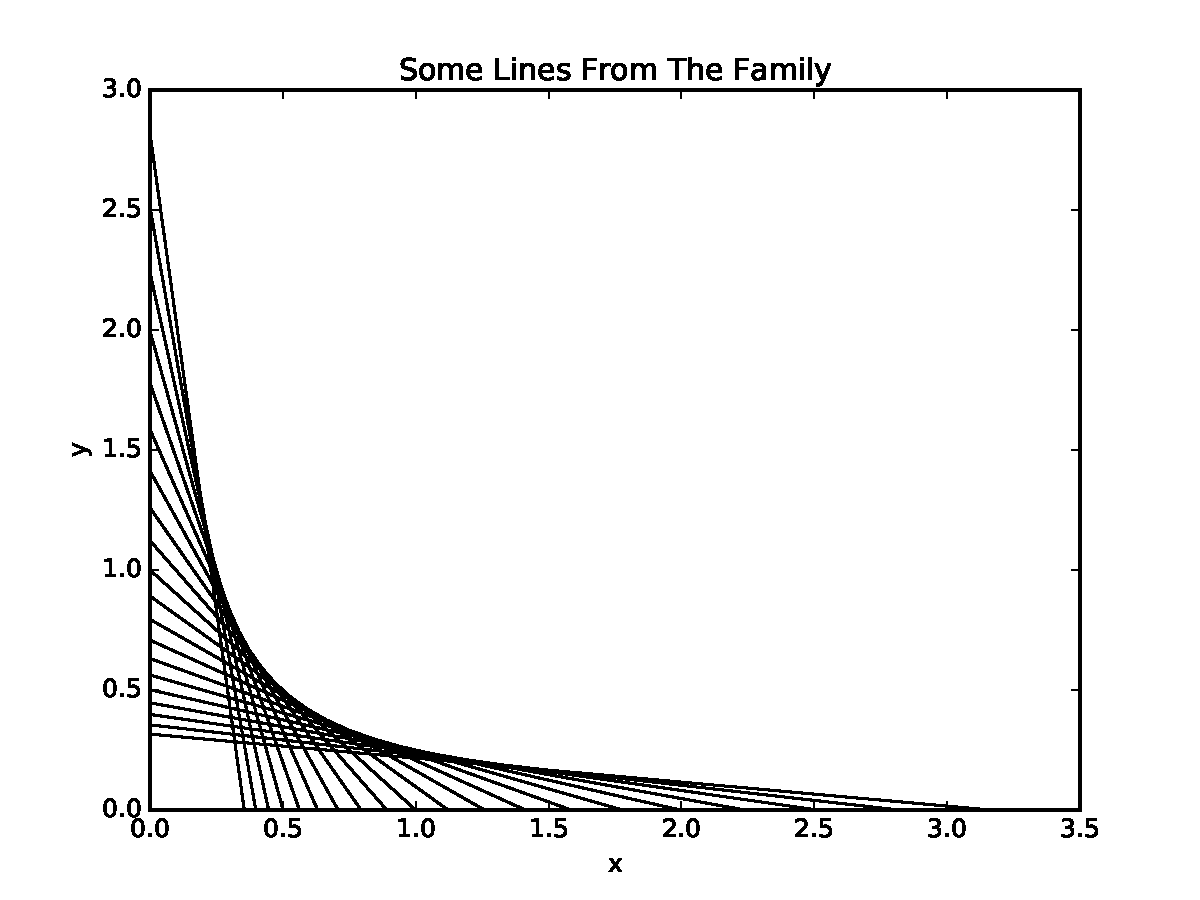
\includegraphics[width = 4.0in]{multiVarDiffCalc/hyperbolaFamily.pdf}

We can see that extemal to the family of lines is a curve concave up in the first quadrant \(\{x, y > 0\}\). In the following figure, you can see the curve superimposed with some of the lines from the family.

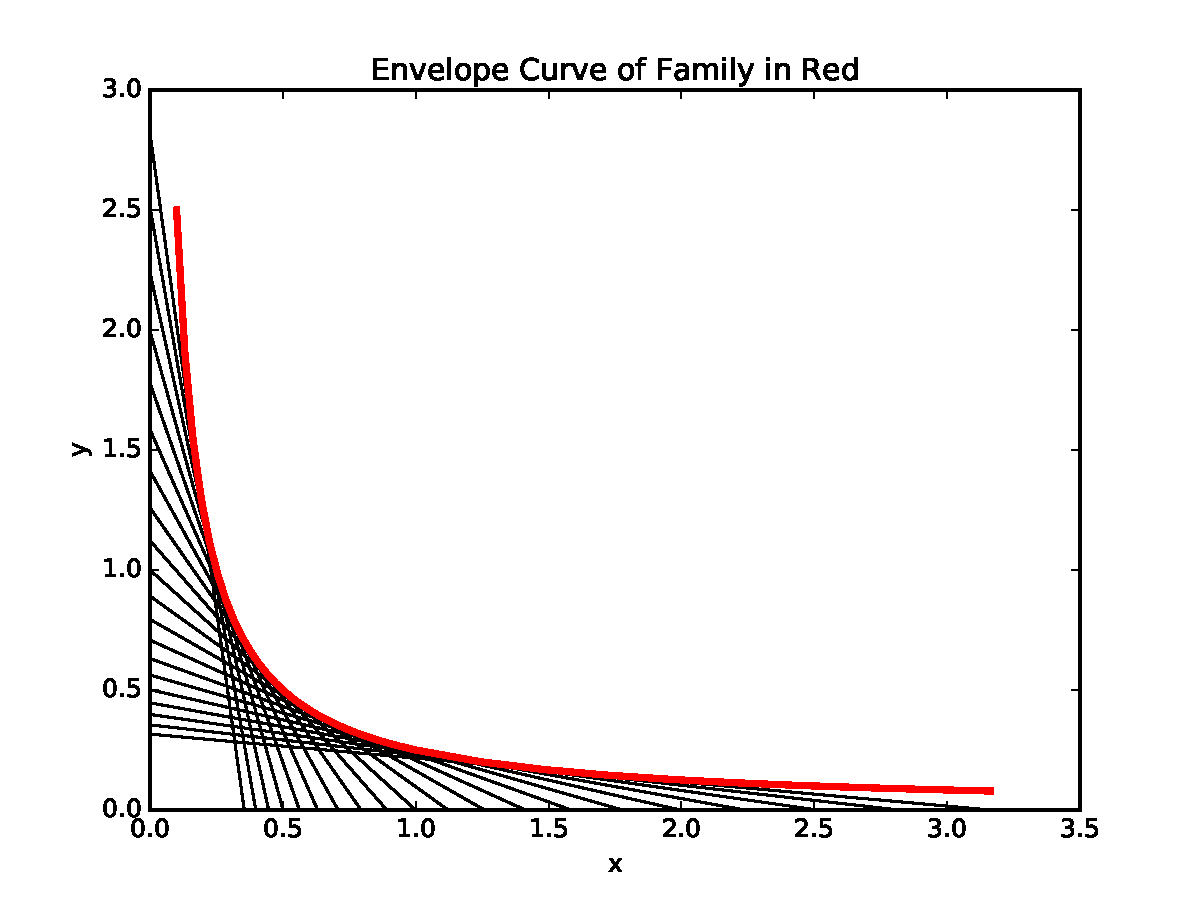
\includegraphics[width = 4.0in]{multiVarDiffCalc/hyperbolaEnvelope.pdf}

\subsubsection*{The Problem}
Let us consider computing the envelope curve \(\gamma(x)\) of the family \(\mathfrak F\). 

\subsubsection*{The Solution}

To compute the envelope curve \(\gamma(x)\), let us consider the auxilliary function
\(g(x,y,s) = \frac{1}{s} x + s y - 1\). Let us see how the Implicit Function Theorem of vector calculus let's us
use \(g(x,y, s)\) to find the exremal envelope curve \(\gamma(x)\). As we discuss this, please consider the similarities to the ordinary first derivative test.

First, consider any point \((x_0, y_0)\) NOT on the extremal envelope curve \(\gamma(x)\), but is touched by some line in \(\mathfrak F\). 
So there is some \(s_0 > 0\) such that \(\frac{1}{s_0} x_0 + s_0 y_0 = 1\); note that this is equivalent to \(g(x_0, y_0, s_0) = 0\). 
Since \((x_0, y_0)\) isn't on the boundary of the region of points touched by lines in \(\mathfrak F\), we know that for any other points \((x_1, y_1)\) close to \((x_0, y_0)\) we may find another line in \(\mathfrak F\) touching \((x_1, y_1)\). 
That is, for every \((x_1, y_1)\) close to \((x_0, y_0)\), we may find \(s_1 > 0\) such that \(g(x_1, y_1, s_1) = 0\).  

This can be summarized as saying that for all points \((x_0, y_0)\) that are touched by a line in \(\mathfrak F\) and also isn't on the envelope \(\gamma\), we can locally solve \(s = S(x,y)\) such that \(g(x, y, S(x, y)) = 0\). Now, you may begin to see the connection to the Implicit Function Theorem.

Recall that the Implicit Function Theorem can only confirm that we CAN locally solve \(s = S(x,y)\) such that \(g(x, y, S(x, y)) = 0\). However, we seek for the extremal points where we CAN'T locally solve. This is similar to the first derivative test of ordinary calculus. Technically, the first derivate test only says when a point is NOT an extemum of a function; then the candidate points for extrema are reduced to some finite list by solving for the vanishing of the derivative.

Here, we are in a similar situation. We solve for a set of candidate points that must contain our extremal curve \(\gamma\). 
It will happen to be the case that our candidate set will allow only one curve and so this must be the envelope.
However, we are being a little reckless here as we haven't proven the curve must exist; we will consider the picture to be very convincing and ignore this technical detail. 

So we seek for when we can't locally solve \(s = S(x,y)\) such that \(g(x, y, S(x, y)) = 0\). The Implicit Function Theorem tells us this will only be possible for those \((x,y,s)\) with \(g(x,y,s) = 0\) and \(\frac{\partial g}{\partial s} (x, y, s) = 0\).

So we look for
\begin{align}
0 & = \frac{\partial g}{\partial s}, \\
&  = -\frac{x}{s^2} + y
\end{align}

We wish to find an equation restricting \(x\) and \(y\); so it is most efficient to solve the above for \(s\). 
Also, from the picture it is clear that we should restrict to \(x, y > 0\). 
Therefore, for \(x, y > 0\), we have \(s = \sqrt{\frac{x}{y}}\). Plugging this into the equation for \(g(x, y, s) = 0\), we get 
\begin{equation}
\sqrt{xy} + \sqrt{xy} - 1 = 0.
\end{equation} 

Therefore, we find that the envelope curve must lie inside the set \(S = \{xy = \frac{1}{4}\}\). However, one will recognize that for each point \(x > 0\), there is only one \(y\) such that \(y \in S\). Therefore, the envelope must be this curve.

So the envelope \(\gamma(x)\) is the curve \(y = \frac{1}{4x}\) for \(x > 0\).  

\subsubsection*{Final Remark}

Note that the set \(S\) is actually a hyperbola. Therefore, the hyperbola can be realized as the envelope of a simple family of straight lines. For this reason, hyperbolas are (approximately) reproducible in "string art": art formed from
straight line segments where each segment is made by tightened string.

\subsection{Differentiable Function With Bounded Non-Continuous Derivatives}

\subsubsection*{Setup}

Functions that are differentiable everywhere do not necessarily have continuous derivatives, even if the derivatives of the function are bounded. For the case of one variable, a classic example is
\begin{equation}
f(x) = \begin{cases}
    x^2 \sin(\frac{1}{x}) & x\neq 0,\\
    0 & x = 0.
    \end{cases}
\end{equation}
Here, the altering of the amplitude by the factor of \(x^2\) forces the function to be differentiable at \(x = 0\) and \(f'(0) = 0\). This can be checked by directly applying the definition of differentiability. However, the derivative \(f'(x)\) alternates infinitely between values close to \(f' = -1\) and \(f' = 1\) as \(x \to 0\). Therefore, the function does not have continuous derivatives.

However, one may wonder if this "infinite frequency oscillation" is necessary. In this example, we show that this is unnecessary in two-dimensions. That is, we construct a function \(u(x,y)\) that is 
differentiable everywhere, has bounded derivatives, and does not have continuous derivatives at \((0,0)\).

\subsubsection*{The Problem}

Find a simple function \(u(x,y)\) such that \(u\) is differentiable on \(\mathbb R^2\), the derivatives of \(u\) are bounded, and at least one of the derivatives of \(u\) is NOT continuous at \((0,0)\).

\subsubsection*{The Solution}

First let us consider a phenomenon in one-variable calculus. If \(g(x)\) is a differentiable function with bounded derivatives: \(|g'| \leq M\), then for any constant \(\lambda > 0\) the function
\(h(x) = \lambda g\left(\frac{x}{\lambda}\right)\) has the same bound for its derivatives, i.e. \(|h'| \leq M\). This is easily proved using the chain rule:
\begin{align}
h'(x) & = \lambda \frac{d}{dx} \left( g\left(\frac{x}{\lambda}\right)\right), \\
    & = \lambda g'\left(\frac{x}{\lambda}\right) \frac{1}{\lambda}, \\
    & = g'\left(\frac{x}{\lambda}\right). 
\end{align}
Therefore, if \(|g'| \leq M\), then \(|h'| \leq M\) too. 

So the idea is that we can construct a function \(u(x,y)\) by setting \(u(x,y) = (x^2 + y^2) h\left(\frac{x}{x^2 + y^2}\right)\) for an appropriate function \(h(x)\). What properties should we require
of \(h(x)\)? First, let's check what is necessary for bounded derivates. Although we were guided by our idea in one-variable differentiation, we must now explicitly check that everything works out okay
since our factor \(x^2 + y^2\) isn't actually constant. 

First, let's calculate the \(x\)-derivative when \((x,y) \neq (0, 0)\):
\begin{align}
\frac{\partial u}{\partial x} & = 2x h + (x^2 + y^2) h' \left(\frac{1}{x^2 + y^2} - \frac{2x^2}{(x^2 + y^2)^2}\right), \\
    & = 2xh + h' - h' \frac{x^2}{x^2 + y^2}. 
\end{align}

Now, let's calculate the \(y\)-derivative when \((x,y) \neq (0,0)\):
\begin{align}
\frac{\partial u}{\partial y} & = 2yh + (x^2 + y^2) h' \frac{2xy}{(x^2 + y^2)^2}, \\
    & = 2yh + h'\frac{2xy}{x^2 + y^2}.
\end{align}

Therefore, we see that the derivatives \(u_x\) and \(u_y\) will be bounded for \((x,y) \neq (0,0)\) when the function \(h(x)\) and its derivative \(h'(x)\) are both bounded; note that expressions like
\(\frac{x^2}{x^2 + y^2}\) and \(\frac{2xy}{x^2 + y^2}\) are bounded for points away from the origin because they are invariant under scaling (i.e. homogeneous of order 0).

Finally, when \(h(x)\) is bounded, the fact that we mulitply \(h\) by \(x^2 + y^2\) to construct \(u\) implies that \(u\) will be differentiable at the origin and that \(u_x(0,0) = u_y(0,0) = 0\).
Now, focus on the expression \(h' \frac{2x^2}{x^2 + y^2}\) in the expression for \(u_x\). If we approach the origin along \(y^4 = x\), then
\begin{align}
h'\left(\frac{x}{x^2 + y^2}\right) & = h'\left(\frac{\sqrt{x}}{x^{3/2} + 1}\right) ,\\
    & \to h'(0).
\end{align} 
Furthermore as we approach the origin along \(y^4 = x\), 
\begin{align}
\frac{x^2}{x^2 + y^2} & = \frac{x^{3/2}}{x^{3/2} + 1}, \\
    & \to 0. 
\end{align}
Therefore, as we approach the origin along \(y^4 = x\), we have that \(u_x \to h'(0)\). So we will want \(h'(0) \neq 0\), e.g. \(h'(0) = 1\).

Let us recap our requirements for \(h(x)\).
\begin{itemize}
\item The function \(h(x)\) is differentiable with continuous derivatives on \(\mathbb R\)
\item The values of the function \(h(x)\) and its derivative \(h'(x)\) are both bounded.
\item At \(x = 0\), we have \(h'(0) = 1\).
\end{itemize}

A function that meets all of these requirements is \(h(x) = \frac{x}{1 + x^2}\). So our function \(u(x,y)\) is
\begin{align}
u(x,y) & = (x^2 + y^2) h\left(\frac{x}{x^2 + y^2}\right), \\
    & = (x^2 + y^2) \frac{x}{(x^2+y^2)(1 + x^2 (x^2 + y^2)^{-2})}, \\
    & = \frac{x(x^2 + y^2)^2}{(x^2 + y^2)^2 + x^2}.
\end{align}

\subsection{Maximizing Likelihood for a Three Step Markov Process}

\subsubsection*{The Setup : The Constraints}

\newcommand{\flip}[1]{\overline{#1}}

We have three random variables \(X_1\), \(X_2\), and \(X_3\) where each \(X_i = 0\) or \(X_i = 1\). The order
of the variables matter, and we think of them as randomly being chosen in sequence according to their indices
one, two, or three. 

So there are eight possible outcomes according to the two possible values for each \(X_i\); we label these
outcomes as \(X_1X_2X_3\), e.g. \(000\) or \(110\). We label the probabilities of the outcomes according to these  
possibilities, e.g. \(p_{000}\) or \(p_{110}\). We think of the probabilities forming a vector 
\(\vec p \in \mathbb R^8\), i.e. the vector \(\vec p = (p_{000}, p_{001}, ..., p_{111})\). 

Finally, one more notation we will use. We will use \(\flip i\) to denote the other value of \(0\) or \(1\) that 
is not \(i\); i.e. if \(i = 1\) then \(\flip i = 0\).

To be a three step Markov process, the transition from \(X_2\) to \(X_3\) needs to depend only on \(X_2\) and
not on the entire history, i.e. not depend on \(X_1\) and \(X_2\). In terms of probabilities, this is
expressed as 
\begin{equation}
P(X_3 = k | X_1 = i, X_2 = j) = P(X_3 = k | X_2 = j).
\end{equation}
Applying Bayes' formula to both sides of this equation, we get
\begin{equation}
\frac{p_{ijk}}{\sum_\gamma p_{ij\gamma}} 
= \frac{\sum_\alpha p_{\alpha jk}} {\sum_{\alpha, \gamma} p_{\alpha j\gamma} }.
\end{equation}
We can rewrite this as 
\begin{equation}
p_{ijk} \sum_{\alpha, \gamma} p_{\alpha j\gamma} =
     \left(\sum_\alpha p_{\alpha jk}\right) \left( \sum_\gamma p_{ij\gamma} \right).
\end{equation}
Next, let's expand the sums over \(\gamma\) as sums over the values \(k\) and \(\flip k\); we get
\begin{equation}
p_{ijk}\sum_\alpha p_{\alpha jk} + p_{ijk} \sum_\alpha p_{\alpha j\flip k} =
p_{ijk} \sum_\alpha p_{\alpha jk} + p_{ij\flip k} \sum_\alpha p_{\alpha jk}.
\end{equation}
Cancelling terms we get
\begin{equation}
p_{ijk} \sum_\alpha p_{\alpha j\flip k} = p_{ij\flip k} \sum_\alpha p_{\alpha jk}.
\end{equation}
Now expand the sum over \(\alpha\) as a sum over the values \(i\) and \(\flip i\), we get
\begin{equation}
p_{ijk} p_{ij\flip k} + p_{ijk} p_{\flip ij\flip k} = p_{ij\flip k} p_{ijk} + p_{ij\flip k} p_{\flip ijk}.
\end{equation}
Again, cancelling terms we get
\begin{equation}
p_{ijk} p_{\flip ij\flip k} = p_{ij\flip k} p_{\flip ijk}.
\end{equation}

Now, at first this appears to be eight different equations, one for each possible choice of \((i, j, k)\). 
However, we will now show that it is actually just two different equations without doing a brute force
plug and check.

First, notice that the equation is exactly the same if we make the substitution \(i \to \flip i\); the effect
is to merely switch the left and right hand side of the equation. Therefore, the equation is the same no matter
which value of \(i\) we choose. So let us choose \(i = 0\).

Similarly, using the substitution \(k \to \flip k\), we can choose \(k = 0\). Both of these choices give
\begin{equation}
p_{0j0} p_{1j1} = p_{0j1} p_{1j0},
\end{equation}
for either \(j = 0\) or \(j = 1\). It is not very hard to see that we get different equations for each
different value of \(j\). 

Therefore, we find that the constraints for \(\vec p\) to be a three step Markov process are exactly the
four following constraints: 
\begin{equation}
\begin{cases}
p_{ijk} \geq 0, \\
\sum_{\alpha, \beta, \gamma} p_{\alpha\beta\gamma} = 1, \\
p_{000} p_{101} = p_{001} p_{100}, \\ 
p_{010} p_{111} = p_{011} p_{110}.
\end{cases}
\end{equation}
All probability vectors \(\vec p \in \mathbb R^8\) that belong to three step Markov processes are exactly 
the probability vectors \(\vec p\in \mathbb R^8\) that satisfy all of the above constraints. 

\subsection*{The Setup: Maximizing Likelihood}

We are interested in creating statistical estimates for the different \(p_{ijk}\) based on data recording
sample counts \(n_{ijk}\); that is, we run \(N\) independent trials, and \(n_{ijk}\) is the 
number of times we see outcome \(X_1 = i\), \(X_2 = j\), and \(X_3 = k\). We denote the collection of
all the \(n_{ijk}\) as a vector \(\vec n\) similarly to how we used \(\vec p\) above. 

First, let us briefly discuss the notion of likelihood. For the notion of likelihood, you consider the
data \(\vec n\) to be fixed, and we consider varying the probabilities of our model \(\vec p\). The 
likelihood is defined as the probabilitiy \(l(\vec p) = P(\vec n | \vec p) \) for our three step Markov
model. Assuming the trials are independent, we have
\begin{equation}
l(\vec p) = \prod_{\alpha, \beta, \gamma} (p_{\alpha\beta\gamma})^{n_{\alpha\beta\gamma}}.
\end{equation} 
The term "likelihood" is used instead of probability, because \(l(\vec p)\) does not in general represent
a probability distribution on \(\vec p\).

The idea is that a good estimate of the true probabilities should come from finding \(\vec p\) that
maximizes the likelihood \(l(\vec p\). 

Next note that maximizing likelihood is equivalent to maiximizing the logarithm of likelihood; however,
the latter has a nicer form. So let \(L(\vec p) = \log(l(\vec p))\). We see that
\begin{equation}
L(\vec p) = \sum_{\alpha, \beta, \gamma} n_{\alpha\beta\gamma} \log(p_{\alpha\beta\gamma}).
\end{equation}

Now, recall that those \(\vec p\) that represent three step Markov processes are exactly those \(\vec p\) 
satisfying four constraints. So we are lead to a constrained maximization problem. We will assume that
the maximum occurs at the interior of the constraints, i.e. \(p_{ijk} > 0\) for all \((i, j, k)\). 

\subsubsection*{The Problem}

Let the data \(n_{ijk}\) be fixed. Assume that the maximum of the following constrained problem occurs at \(p_{ijk} > 0\) for all \((i, j, k)\):
\begin{equation}
\begin{cases}
\text{maximize } L(\vec p) = \sum_{\alpha, \beta, \gamma} n_{\alpha\beta\gamma} \log p_{\alpha\beta\gamma}, \\
\sum_{\alpha, \beta, \gamma} p_{\alpha\beta\gamma} = 1, \\
p_{0j0} p_{1j1} = p_{0j1} p_{1j0}, & \text{ for } j \in \{0, 1\}.
\end{cases}
\end{equation}

Find the \(p_{ijk}\) where the maximum occurs in terms of the data \(n_{ijk}\).


\section{Multivariable Integral Calculus}

\subsection{Function Not Satisfying Fubini's Theorem}

\subsubsection*{Set Up}

Here we consider Fubini's theorem in two-dimensions.

Fubini's theorem tells us two things:
\begin{itemize}
\item When we know we can compute a two-dimensional integral as a repeated application of one-dimensional integration over the variables \(x\) and \(y\).

\item When we know the order of the repeated one-dimensional integration over \(x\) and \(y\) doesn't depend on the order of integrating over \(x\) and \(y\). 

\end{itemize}

We will consider the problem of finding a simple function that doesn't satisfy Fubini's theorem. In particular, the result of applying the repeated 
one-dimensional integration will depend on the order of \(x\) and \(y\). We will aim to find a simple elementary function, and we will keep the domain of integration
simple, i.e. the square \(S = \{0 \leq x \leq 1 \text{ and } 0 \leq y \leq 1\}\).

As a hint as to how this process will work, let us recall the fact that for a convergent series \(\sum_i a_i\), the limit of the partial sums is independent of the order of
the sum when the series is absolutely convergent, i.e. \(\sum_i |a_i| < \infty\). For our problem of finding an appropriate function \(u(x,y)\), we are then lead to consider
finding a function \(u(x,y)\) that satisfies the following:
\begin{itemize}
\item The function \(u(x,y)\) takes positive and negative values. 
\item The integral of the aboslute value of \(u\) is not convergent, i.e. \(\iint_s |u| \dA = \infty\).
\item The integrals of the positive and negative parts of the function must cancel out in some way such that the repeated integration gives nice finite values despite
the fact that \(\iint_s |u| \dA = \infty\).
\end{itemize}


\subsubsection*{The Problem}

Find a nice elementary function \(u(x, y)\) defined on the square \(s = \{0 \leq x \leq 1 \text{ and } 0 \leq y \leq 1\}\) such that \(u(x,y)\) doesn't satisfy Fubini's theorem in the following sense:
\begin{itemize}
\item Both of the repeated integrals
\begin{equation}
\int\limits_0^1 \int\limits_0^1 u(x,y) \dx \dy,
\end{equation}
and
\begin{equation}
\int\limits_0^1 \int\limits_0^1 u(x,y) \dy \dx,
\end{equation}
exist and are finite.
\item However, the repeated integrals mentioned above are NOT equal.
\end{itemize}

\subsubsection*{Solution}

To keep things simple, we find a function \(u(x,y)\) that blows up to both \(\pm \infty\) at the corner \((0,0)\). First let us observe that the function 
\begin{equation}
f(x,y) = \frac{-1}{(x+y)^2}
\end{equation}
has \(\iint_S |f| \dA = \infty\); you can quickly see that convergence of this integral is suspect because \(|f|\) of order \(r^{-2}\) as the radius \(r \to 0\). This is the edge case of convergence
for two-dimensions (recall that the area element for polar coordinates in two-dimensions includes an extra \(r\), i.e. \(\dA = r d\theta dr\)). 

However, \(f(x,y)\) is always negative inside the square \(S\); so we won't get the cancellation of positive and negative parts that we desire. To fix this we set up \(u(x,y)\) to be a difference
of \(f(x,y)\) and a similar function. First, let \(A, B\) be constants that we will determine later. Then we use
\begin{equation}
u(x,y) = \frac{1}{(Ax + By)^2} - \frac{1}{(x+y)^2} .
\end{equation}

We need that \(u\) takes positive and negative values in \(S\). To make sure \(u\) is always defined in \(S\) we will restrict to considering \(A, B > 0\).

Next, consider the values of \(u\) along the line \(\{x + y = 1\}\). This line joins two corners of \(S\), i.e. \((0,1)\) and \((1,0)\). We will design \(A\) and \(B\) to make
sure \(u\) has opposite signs at these two corners. To do so, we need to compare the sizes of \(Ax + By\) and \(x + y\) at these two corners.

To get opposite signs, we need that \(Ax + By\) is above \(1\) at one of these two corners and below \(1\) at the other corner. At \((0,1)\), \(Ax + By = B\) and at \((1,0)\), \(Ax + By = A\).
So we can choose \(A\) is above \(1\) and \(B\) is below \(1\). A convenient choice is \(A = 2\) and \(B = 1/2\) (if you dive deeper into the construction, you will find that the reciprocal nature of \(A\) and \(B\) is also necessary, but we won't go into detail on this). 

So we have that
\begin{equation}
u(x,y) = \frac{1}{(2x + y/2)^2} - \frac{1}{(x+y)^2}.
\end{equation}
Let us verify that this function \(u(x,y)\) satisfies the conditions on the repeated integrals that we are looking for.

First, note that for any \(y > 0\), we have
\begin{align}
\int\limits_0^1 \frac{1}{(2x + y/2)^2} - \frac{1}{(x+y)^2} \dx & = \left.\frac{1}{x+y} - \frac{1}{2(2x + y/2)}\right|^1_{x = 0}, \\ 
    & = \frac{1}{1 + y} - \frac{1}{y} - \frac{1}{4+y} + \frac{1}{y}, \\
    & = \frac{1}{1+y} - \frac{1}{4+y}.
\end{align}
So we get that
\begin{align}
\int\limits_0^1 \left(\int\limits_0^1 \frac{1}{(2x + y/2)^2} - \frac{1}{(x+y)^2} \dx\right) \dy & = \int\limits_0^1 \frac{1}{1+y} - \frac{1}{4 + y} \dy, \\
    & = \left. \log(1 +y) - \log(4 + y)\right|_{y = 0}^1, \\
    & = \log(2) - \log(1) - \log(5) + \log(4), \\
    & = 3\log(2) - \log(5). 
\end{align}

Now, let us consider the other iterated integral. First, for any \(x > 0\), we have that
\begin{align}
\int\limits_0^1 \frac{1}{(2x + y/2)^2} - \frac{1}{(x+y)^2} \dy & = \left.\frac{1}{x+y} - \frac{2}{2x + y/2}\right|_{y = 0}^1, \\
    & = \frac{1}{x+1} - \frac{1}{x} -\frac{2}{2x+1/2} + \frac{2}{2x}, \\ 
    & = \frac{1}{x+1} - \frac{2}{2x+1/2}.
\end{align}
So we have that
\begin{align}
\int\limits_0^1 \left(\int\limits_0^1 \frac{1}{(2x + y/2)^2} - \frac{1}{(x+y)^2} \dy\right) \dx & = \int\limits_0^1 \frac{1}{x+1} - \frac{2}{2x+1/2} \dx, \\
    & = \left. \log(x+1) - \log(2x + 1/2)\right|_{x = 0}^1, \\
    & = \log(2) - \log(1) - \log(5/2) + \log(1/2), \\
    & = \log(2) - \log(5). 
\end{align}
And so we see the repeated integrals are finite, but do NOT match.


\bibliography{references}{}
\bibliographystyle{plain}
\end{document}
